\begin{surferPage}[Dubbele kegel]{Een dubbele kegel}
  In de introductie tot deze galerij werd reeds uitgelegd wat gladde of \textit{niet-singuliere} oppervlakken zijn. Voorbeelden hiervan zie je op de linkse en middelste afbeelding hieronder: een boloppervlak en een torus.
    \begin{center}
      \begin{tabular}{@{}c@{}c@{}c@{}c@{}}
        \begin{tabular}{@{}c}
          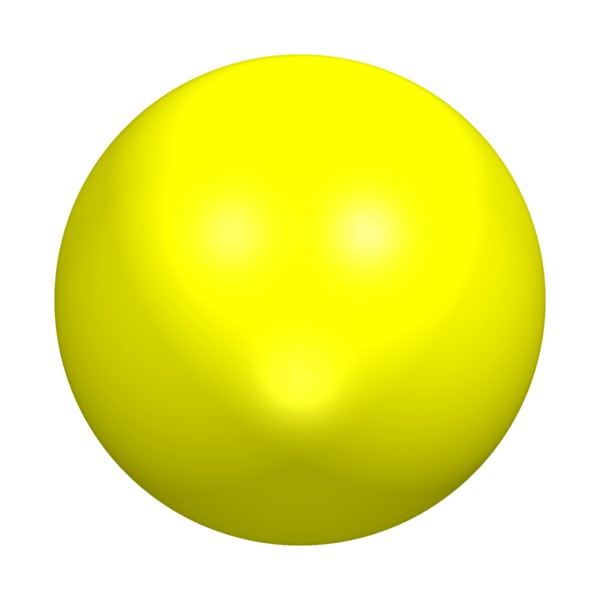
\includegraphics[width=1.4cm]{kugel}
        \end{tabular}
        &
        \begin{tabular}{@{}c}
          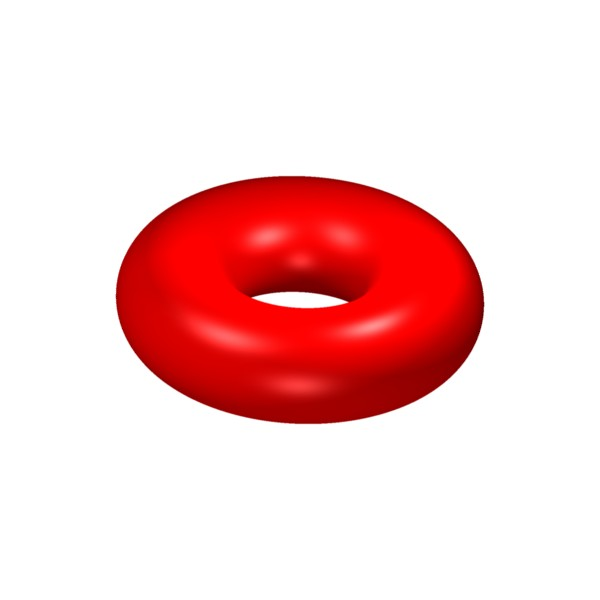
\includegraphics[width=1.4cm]{torus}
        \end{tabular}
        &
        \begin{tabular}{c@{}}
          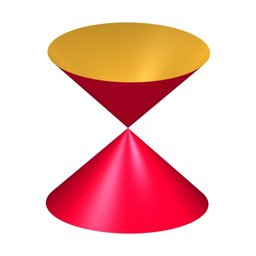
\includegraphics[width=1.4cm]{kegel}
        \end{tabular}
      \end{tabular}
    \end{center}
     De dubbele kegel (rechtse afbeelding) toont de eenvoudigste singulariteit; het is de enige die kan beschreven worden met een vergelijking van graad $2$:
    \[x^2+y^2-z^2=0.\]
    Als we deze vergelijking lichtjes veranderen door de $0$ te vervangen door een kleine waarde $a\neq 0$ verandert de dubbele kegel in \'e\'en van de twee types hyperbolo\"ides, afhankelijk van het teken van $a$:
    \begin{center}
      \begin{tabular}{@{}c@{\ }c@{\ }c@{\ }c@{\ }c@{}}
        \begin{tabular}{@{}c@{}}
          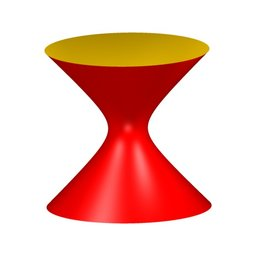
\includegraphics[width=1.2cm]{A1pm_2}
        \end{tabular}
        &
        $\leftarrow$
        &
        \begin{tabular}{@{}c@{}}
          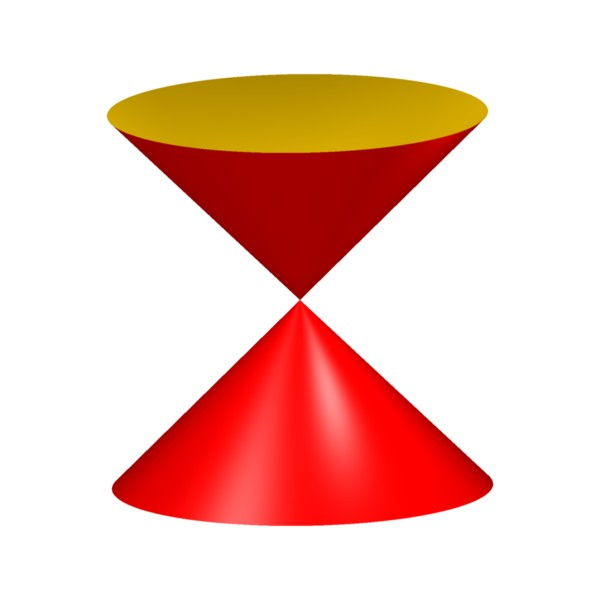
\includegraphics[width=1.2cm]{A1pm_1} 
        \end{tabular}
        &
        $\rightarrow$
        &
        \begin{tabular}{@{}c@{}}
          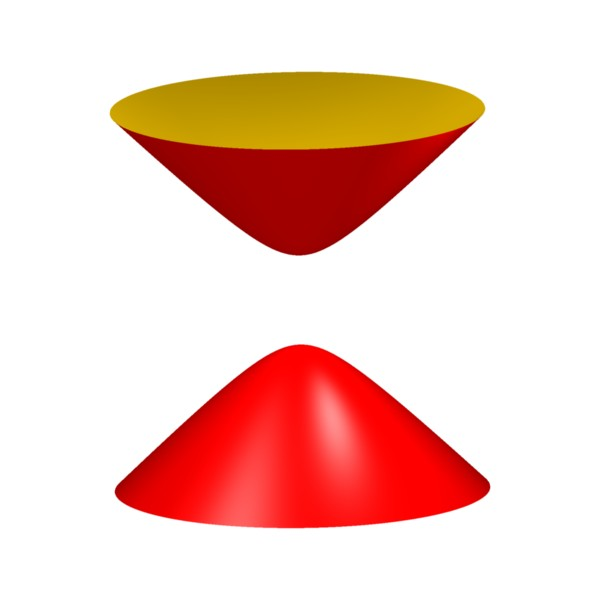
\includegraphics[width=1.2cm]{A1pm_0}
        \end{tabular}
      \end{tabular}
    \end{center}
   Een oppervlak van graad $2$ kan niet meer dan \'e\'en singulariteit hebben, i.e.\ $\mu(2)=1$.
\end{surferPage}
